\FloatBarrier
\subsection{Caso d'uso UC 0: \progetto (SDK)}
\label{Caso d'uso UC 0: \progetto (SDK)}
\begin{figure}[ht]
	\centering
	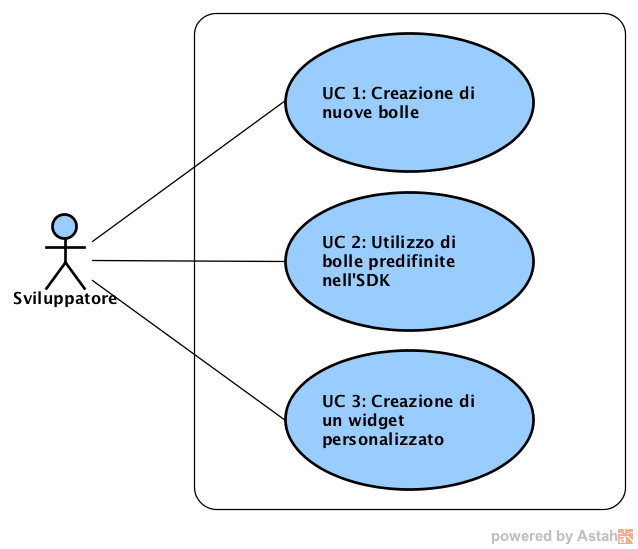
\includegraphics[scale=0.80]{Usecases/img/Monolith.png}
	\caption{Caso d'uso UC 0: \progetto(SDK)}
\end{figure}

\FloatBarrier
\begin{itemize}
\item \textbf{Attori:} Sviluppatore.
\item \textbf{Descrizione:} Tramite l'\termine{SDK} lo sviluppatore vuole:
	\begin{itemize}
	\item{Creare una nuova bolla utilizzando i widget dell'\termine{SDK}.}
	\item{Utilizzare una bolla predefinita.}
	\item{Creare un nuovo widget.}
	\end{itemize}
\item \textbf{Precondizione:} Lo sviluppatore ha accesso all'\termine{SDK}.
\item \textbf{Postcondizione:} Lo sviluppatore ha creato del codice eseguibile.
\item \textbf{Scenario Principale:}
	\begin{itemize}
	\item{Creazione di nuove bolle utilizzando i widget dell'\termine{SDK} (UC 1).}
	\item{Utilizzo di bolle predefinite nell'\termine{SDK} (UC 2).}
	\item{Creazione di un widget personalizzato (UC 3).}
	\end{itemize}
\end{itemize}